\chapter[Distances Between Distributions]{Distances Between Distributions: Total Variation and Kullback--Leibler}
\label{ch:distances}

\begin{chaptergoals}
\begin{itemize}[nosep]
\item Why `the estimate is close to the truth' should be measured between distributions and not between parameters, and an example where a parameter difference of $0.01$ means almost nothing in one place and a great deal in another.
\item Total variation: the largest disagreement between two distributions over all events, equal to the area between their densities. What it says about tests: the best possible test between two distributions has $\alpha + \beta = 1 - \TV$.
\item Why total variation, for all its good properties, can't be estimated by an average of the data.
\item The Kullback--Leibler divergence: the average evidence one observation supplies against the wrong distribution. Its properties, its asymmetry, why it adds up over independent observations, and why near the truth it is a parabola.
\item Estimating the KL divergence by the Law of Large Numbers, and the discovery that minimizing the estimate is maximizing the likelihood.
\item What an estimator estimates when the model is wrong: the member of the family closest to the truth in KL. For the Gaussian family that is the member with the right mean and variance.
\end{itemize}
Part III judged estimators that were handed to you. This chapter is the first step toward producing them: it says what `close' means, and the answer leads straight to maximum likelihood in \cref{ch:likelihood}.
\end{chaptergoals}

\section{What `close to the truth' should mean}
\label{sec:dist-close}

Go back to the setup of \cref{ch:models}.
You have a statistical model $(E, (\Pr_\theta)_{\theta \in \Theta})$, data $\Xton \iid \Pr_{\theta^*}$ from a true parameter $\theta^*$ that you don't know, and an estimator $\hat{\theta}_n$.
What would it mean for $\hat{\theta}_n$ to be a good estimator?

The answer of \cref{ch:estimators} was that $\hat{\theta}_n$ should be close to $\theta^*$ as numbers: small bias, small variance, small quadratic risk $\E[(\hat{\theta}_n - \theta^*)^2]$.
That is a fine answer when the parameter is the thing you care about, like the share of couples who turn right.
But a parameter is a label for a distribution.
What you actually use a fitted model for is its distribution: the probability it assigns to an interval, a tail, a range of outcomes.
So the question you'd really like answered is whether the fitted distribution $\Pr_{\hat{\theta}_n}$ is close to the true one $\Pr_{\theta^*}$, in the sense that for every event $A$,
\[
\Pr_{\hat{\theta}_n}(A) \approx \Pr_{\theta^*}(A).
\]
If that holds, every probability you compute from the fitted model is about right, and that is the whole point of fitting it.

\begin{intuition}[a parameter difference has no fixed meaning]
Is a difference of $0.01$ between two parameters small?
It depends on where in the parameter space it happens.
Two Gaussians with standard deviation $1$ whose means differ by $0.01$ are, for every practical purpose, the same distribution: no event has probabilities under the two that differ by more than $0.004$.
Two Gaussians with mean $0$ whose standard deviations are $0.01$ and $0.02$ also have parameters $0.01$ apart, and they are obviously different distributions: one is twice as wide as the other, and there is an event whose probability is $0.32$ higher under one than under the other.
\Cref{fig:paramvsdist} draws both.
\end{intuition}

\begin{figure}[htbp]
\centering
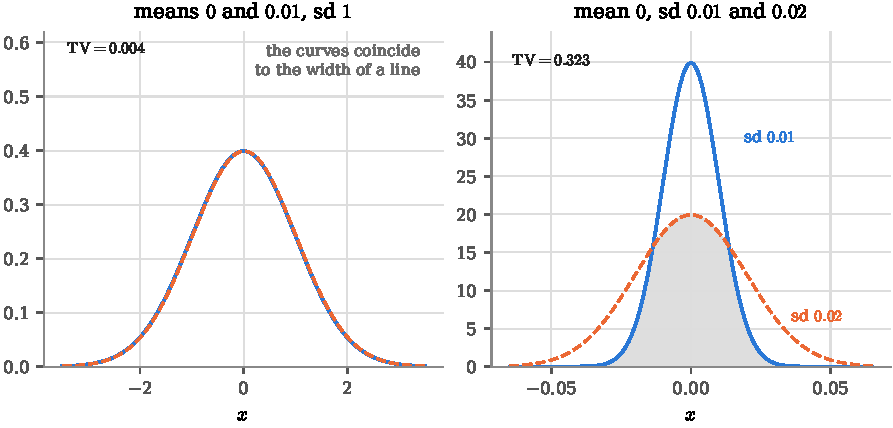
\includegraphics[width=\textwidth]{fig_param_vs_dist}
\caption{Two pairs of Gaussians whose parameters differ by $0.01$. Left: means $0$ and $0.01$, standard deviation $1$; the curves coincide to the width of a line and the total variation distance is $0.004$. Right: mean $0$, standard deviations $0.01$ and $0.02$; the curves share only the gray area, $0.677$, so the total variation distance is $0.323$.}
\label{fig:paramvsdist}
\end{figure}

There is a second reason to measure closeness between distributions, and it matters as much as the first.
\Cref{sec:models-wellspecified} asked whether the model is well-specified, whether the true distribution is in the family at all.
If it isn't, there is no $\theta^*$, and `the distance from $\hat{\theta}_n$ to $\theta^*$' has no meaning.
A distance between distributions still has one: you can ask which member of the family is closest to the truth, even when none of them is the truth.
\Cref{sec:dist-projection} answers that question.

The chapter builds two such measures.
The first, total variation, is the natural one, and it is a true distance.
The second, the Kullback--Leibler divergence, is not a true distance, and it is the one statistics uses, for a reason that takes \cref{sec:dist-tv-estimate} to explain.

\section{Total variation}
\label{sec:dist-tv}

The requirement `$\Pr(A) \approx \Qr(A)$ for every event $A$' already contains a definition.
Look at all the events, find the one on which the two distributions disagree most, and call that disagreement the distance.

\begin{definition}[Total variation distance]
\label{def:tv}
Let $\Pr$ and $\Qr$ be two probability distributions on the same sample space $E$.
The \textbf{total variation distance} between them is
\[
\TV(\Pr, \Qr) = \max_{A \subset E} \abs{\Pr(A) - \Qr(A)},
\]
the largest difference between the probabilities they assign to one event.
\end{definition}

\begin{inwords}
\textbf{In words.} Run through every question you could ask about one draw (is it positive? is it between $2$ and $3$? is it even?) and record how differently the two distributions answer. The total variation distance is the worst case. If it is $0.01$, no question you could ever ask gets answers more than one percentage point apart. That is exactly the guarantee you want from a fitted model: every probability it reports is within $\TV$ of the true one.
\par\smallskip
\textbf{For the kiss data.} One couple either turns right or doesn't, so there are four events: nothing, `right', `left' and everything. Compare $\Bern(0.645)$, the fitted distribution, with $\Bern(\frac12)$, `no preference'. The empty event and the whole space get probabilities $0$ and $1$ from both. `Right' gets $0.645$ and $0.5$; `left' gets $0.355$ and $0.5$. The largest difference is $0.145$, so $\TV = 0.145$. As a natural frequency: of $1{,}000$ couples, the fitted model predicts $645$ right turns and `no preference' predicts $500$; the two descriptions disagree about $145$ couples in a thousand.
\end{inwords}

For a sample space with four events the maximum is easy.
For a sample space like $\real$ there are uncountably many events, and searching over them is not a calculation anyone wants to do.
The next result turns the maximum into a sum or an integral.

\begin{proposition}[Total variation as an area]
\label{prop:tv-area}
If $\Pr$ and $\Qr$ have PMFs $p$ and $q$ on a discrete $E$,
\[
\TV(\Pr, \Qr) = \frac12 \sum_{x \in E} \abs{p(x) - q(x)};
\]
if they have densities $p$ and $q$,
\[
\TV(\Pr, \Qr) = \frac12 \int_E \abs{p(x) - q(x)} \, \mathrm{d}x.
\]
The maximum in \cref{def:tv} is attained at the event $A^\star = \{x : p(x) > q(x)\}$, where $\Pr$ puts more mass than $\Qr$.
\end{proposition}

\coreproof{The event that favors $\Pr$ most collects every point where $p$ beats $q$ and no other point. Its advantage is the area of the region where $p$ is above $q$; the region where $q$ is above $p$ has the same area, since both densities have total mass $1$. Half the total area between the curves is therefore the area of either piece.}
\begin{proof}
The discrete case; the continuous one replaces sums by integrals.
Split $E$ into $A^\star = \{p > q\}$ and its complement $\{p \leq q\}$.
For any event $A$,
\[
\Pr(A) - \Qr(A) = \sum_{x \in A} \big(p(x) - q(x)\big) \leq \sum_{x \in A \cap A^\star} \big(p(x) - q(x)\big) \leq \sum_{x \in A^\star} \big(p(x) - q(x)\big) = \Pr(A^\star) - \Qr(A^\star).
\]
The first inequality drops the points of $A$ where $p - q \leq 0$, which can only increase the sum; the second adds the points of $A^\star$ that $A$ missed, where $p - q > 0$, which can only increase it again.
The same argument with $\Pr$ and $\Qr$ exchanged gives $\Qr(A) - \Pr(A) \leq \Qr(A^{\star c}) - \Pr(A^{\star c})$.
Both $p$ and $q$ sum to $1$, so
\[
\sum_{x \in A^\star} \big(p(x) - q(x)\big) + \sum_{x \notin A^\star} \big(p(x) - q(x)\big) = 1 - 1 = 0,
\]
which says that $\Pr(A^\star) - \Qr(A^\star) = \Qr(A^{\star c}) - \Pr(A^{\star c})$: the area where $p$ is above $q$ equals the area where $q$ is above $p$.
Call this common value $D$.
Every event has $\abs{\Pr(A) - \Qr(A)} \leq D$, and $A^\star$ attains it, so $\TV(\Pr, \Qr) = D$.
Finally $\sum_x \abs{p(x) - q(x)}$ is the sum of the two pieces, $D + D = 2D$, and so $D = \frac12 \sum_x \abs{p(x) - q(x)}$.
\end{proof}

\Cref{fig:tvarea} is the proposition as a picture.
Lay the two densities on top of each other.
Where they overlap, the gray region, they agree.
Where they don't, the area splits into two pieces of equal size, one where $p$ is above and one where $q$ is above, and the total variation distance is the area of either piece.
Equivalently, $1 - \TV$ is the area of the overlap, the probability mass the two distributions share.

\begin{figure}[htbp]
\centering
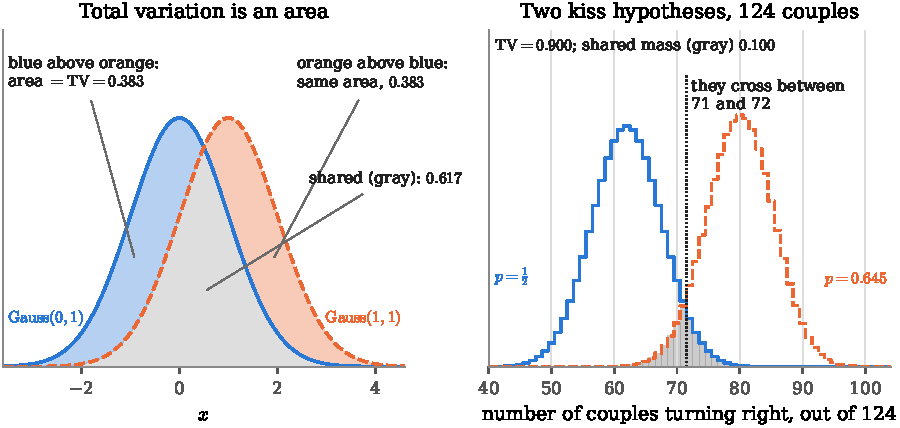
\includegraphics[width=\textwidth]{fig_tv_area}
\caption{Total variation as an area. Left: $\Gauss(0,1)$ and $\Gauss(1,1)$. The blue region, where the first density is above the second, and the orange region, where the second is above the first, have the same area, $0.383$, which is the total variation distance; the gray overlap has area $1 - 0.383 = 0.617$. Right: the distributions of the number of right turns among $124$ couples when $p = \frac12$ and when $p = 0.645$. They share only $0.100$ of their mass (gray), so $\TV = 0.900$, and the two PMFs cross between $71$ and $72$.}
\label{fig:tvarea}
\end{figure}

\begin{worked}[four total variation distances]
\begin{itemize}
\item \textbf{Two Bernoullis.} For $\Bern(p)$ and $\Bern(q)$ the PMFs differ by $\abs{p - q}$ at $1$ and by $\abs{(1-p) - (1-q)} = \abs{p - q}$ at $0$, so
\[
\TV(\Bern(p), \Bern(q)) = \tfrac12\big(\abs{p - q} + \abs{p - q}\big) = \abs{p - q}.
\]
For the kiss data, $\abs{0.645 - 0.5} = 0.145$, as the in-words box found by listing events. For $\Bern(\frac12)$ against $\Bern(\frac1{10})$, $0.4$.
\item \textbf{Two Gaussians with the same variance.} The densities of $\Gauss(0, 1)$ and $\Gauss(\mu, 1)$, $\mu > 0$, cross at the midpoint $\mu/2$, and $A^\star = \{x < \mu/2\}$ is where the first is above. So $\TV = \Pr(Z < \mu/2) - \Pr(Z + \mu < \mu/2) = \Phi(\mu/2) - \Phi(-\mu/2) = 2\Phi(\mu/2) - 1$ for $Z \sim \Gauss(0,1)$. With $\mu = 1$ this is $0.383$, the left of \cref{fig:tvarea}; with $\mu = 0.01$ it is $0.004$, the left of \cref{fig:paramvsdist}.
\item \textbf{An exponential and a uniform.} $\Expo(1)$ has density $e^{-x}$ on $[0, \infty)$, and $\Unif([0,1])$ has density $1$ on $[0,1]$. The two need a common sample space, and $[0, \infty)$ contains both. On $[0,1]$, $1 \geq e^{-x}$; beyond $1$, only the exponential has mass. So
\[
\TV = \frac12 \left( \int_0^1 (1 - e^{-x}) \, \mathrm{d}x + \int_1^\infty e^{-x} \, \mathrm{d}x \right) = \frac12 \left( (1 - 1 + e^{-1}) + e^{-1} \right) = e^{-1} = 0.368.
\]
\item \textbf{Number of right turns.} $\Bin(124, \frac12)$ against $\Bin(124, 0.645)$: half the sum of $125$ absolute differences, computed by machine, is $0.900$. One couple's distributions are $0.145$ apart; $124$ couples' are $0.900$ apart. \Cref{sec:dist-tv-tests} says what that growth means.
\end{itemize}
\end{worked}

\begin{proposition}[Total variation is a distance]
\label{prop:tv-metric}
For distributions $\Pr$, $\Qr$, $\mathbb{V}$ on the same $E$:
\begin{enumerate}[nosep]
\item \textbf{symmetry:} $\TV(\Pr, \Qr) = \TV(\Qr, \Pr)$;
\item \textbf{bounds:} $0 \leq \TV(\Pr, \Qr) \leq 1$, with $\TV = 1$ exactly when there is an event that has probability $1$ under one and $0$ under the other;
\item \textbf{definiteness:} $\TV(\Pr, \Qr) = 0$ only if $\Pr = \Qr$;
\item \textbf{triangle inequality:} $\TV(\Pr, \Qr) \leq \TV(\Pr, \mathbb{V}) + \TV(\mathbb{V}, \Qr)$.
\end{enumerate}
\end{proposition}

\optionalproof{Each property holds for every single event, and taking the maximum over events keeps it.}
\begin{proof}
(1) $\abs{\Pr(A) - \Qr(A)} = \abs{\Qr(A) - \Pr(A)}$.
(2) Every $\abs{\Pr(A) - \Qr(A)}$ is a difference of two numbers in $[0,1]$, so it lies in $[0,1]$. It equals $1$ only if one probability is $1$ and the other is $0$.
(3) If the maximum over events is $0$, every event has the same probability under both, and that is what $\Pr = \Qr$ means.
(4) For each event, $\abs{\Pr(A) - \Qr(A)} \leq \abs{\Pr(A) - \mathbb{V}(A)} + \abs{\mathbb{V}(A) - \Qr(A)}$ by the triangle inequality for numbers \toolkit{sec:math-inequalities}, and each term on the right is at most the corresponding total variation. Take the maximum over $A$ on the left.
\end{proof}

A total variation of $1$ means the two distributions live on separate parts of the sample space: one draw tells you, with certainty, which one it came from.
A total variation of $0$ means they are the same.
Everything else is in between, and \cref{sec:dist-tv-tests} makes `in between' precise.

\begin{bridge}[effect sizes and overlap]
An introductory course measured how far apart two groups are with Cohen's $d$, the difference in means in units of the standard deviation, and called $0.2$ small, $0.5$ medium and $0.8$ large.
For two Gaussians with a common standard deviation, $d$ is a parameter distance, and the second item of the worked example converts it to a distance between distributions: $\TV = 2\Phi(d/2) - 1$.
\Cref{fig:tvcohen} draws the three conventional sizes.
A `large' effect still leaves the two distributions sharing $69\%$ of their mass, and a `small' one leaves them sharing $92\%$.
The shared area $1 - \TV$ is what some texts call the overlapping coefficient, and $\TV$ is the share of each group that has no counterpart in the other.
With equal numbers in the two groups, the best rule for guessing which group one person came from is right with probability $(1 + \TV)/2$, which at $d = 0.8$ is $0.66$.
\end{bridge}

\begin{figure}[htbp]
\centering
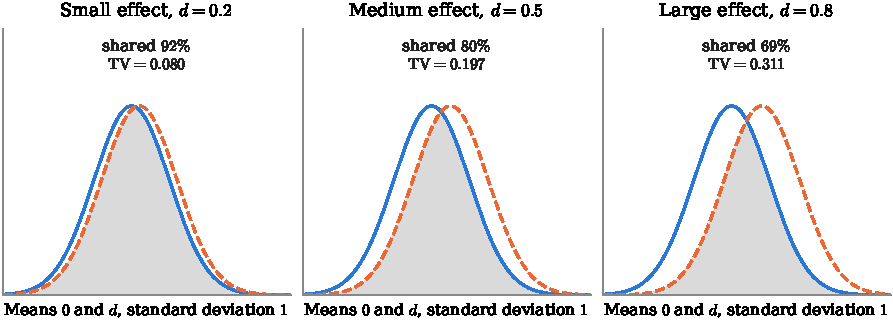
\includegraphics[width=\textwidth]{fig_tv_cohen}
\caption{Cohen's three conventional effect sizes as total variation distances between $\Gauss(0,1)$ (blue, solid) and $\Gauss(d,1)$ (orange, dashed). The shared mass (gray) is $92\%$, $80\%$ and $69\%$; the total variation distances are $0.080$, $0.197$ and $0.311$.}
\label{fig:tvcohen}
\end{figure}

\begin{pitfall}[total variation does not know which outcomes are near each other]
Let $X \sim \Bern(\frac12)$ and $a = 0.001$.
The random variable $X + a$ is $X$ shifted by a thousandth, and any reasonable notion of `close' should call the two distributions close.
Total variation calls them as far apart as two distributions can be: $X$ lives on $\{0, 1\}$, $X + a$ on $\{0.001, 1.001\}$, the event $\{0, 1\}$ has probability $1$ under the first and $0$ under the second, and $\TV = 1$.
Total variation compares probabilities point by point; it has no idea that $0$ and $0.001$ are neighbors.
The same thing happens with the CLT.
\recall{The Central Limit Theorem (\cref{thm:clt}): for iid data with mean $\mu$ and variance $\sigma^2$, $\sqrt{n}(\bar{X}_n - \mu)/\sigma \convd \Gauss(0,1)$.}
For $\Xton \iid \Bern(\frac12)$, $2\sqrt{n}(\bar{X}_n - \frac12) \convd \Gauss(0,1)$, but $2\sqrt{n}(\bar{X}_n - \frac12)$ takes only the $n + 1$ values $2\sqrt{n}(k/n - \frac12)$, a set that has probability $1$ under its own distribution and probability $0$ under any continuous one.
So the total variation distance between the standardized mean and its Gaussian limit is $1$ for every $n$.
Convergence in distribution (\cref{def:convd}) is not convergence in total variation, and it can't be: a discrete distribution is never close to a continuous one in total variation, however finely its mass is spread.
\end{pitfall}

\section{What total variation says about tests}
\label{sec:dist-tv-tests}

Total variation has an operational meaning that makes `in between' concrete: it measures how well data from one distribution can be told apart from data from the other.

Suppose you have to decide, from one draw $X$, whether it came from $\Pr$ or from $\Qr$.
This is the test of \cref{ch:tests-foundations} with $H_0: X \sim \Pr$ and $H_1: X \sim \Qr$, both simple.
A test is an event $R$, the rejection region, and its two errors are $\alpha = \Pr(R)$, rejecting when $\Pr$ is true, and $\beta = \Qr(R^c)$, not rejecting when $\Qr$ is true.
How small can the two errors be together?

\begin{proposition}[The best test and total variation]
\label{prop:tv-best-test}
For every test $R$ of $\Pr$ against $\Qr$,
\[
\alpha + \beta = \Pr(R) + \Qr(R^c) \geq 1 - \TV(\Pr, \Qr),
\]
with equality for the test that rejects where $\Qr$'s density is larger, $R = \{x : q(x) > p(x)\}$.
\end{proposition}

\coreproof{Rewrite $\alpha + \beta$ as $1$ minus the advantage $\Qr(R) - \Pr(R)$ the rejection region gives the alternative. That advantage can never exceed $\TV$, and the region where $q$ beats $p$ achieves it.}
\begin{proof}
$\Qr(R^c) = 1 - \Qr(R)$, so $\alpha + \beta = 1 - \big(\Qr(R) - \Pr(R)\big)$.
By \cref{def:tv}, $\Qr(R) - \Pr(R) \leq \TV(\Pr, \Qr)$ for every event $R$, which gives the inequality.
By \cref{prop:tv-area} with the roles of $\Pr$ and $\Qr$ exchanged, the event $\{q > p\}$ attains the maximum, which gives the equality.
\end{proof}

\begin{intuition}[total variation is distinguishability]
Read \cref{prop:tv-best-test} at its two ends.
If $\TV = 0$, the two distributions are the same, and every test has $\alpha + \beta = 1$ exactly, no better than a test that ignores the data.
If $\TV = 1$, the two live on separate parts of $E$, and the test `reject if $X$ lands in $\Qr$'s part' makes no errors at all.
In between, $1 - \TV$ is the irreducible error: the total of the two error rates that no test, however clever, can get below.
In \cref{fig:tvarea} it is the gray overlap.
A draw that lands in the overlap could have come from either distribution, and that is where every test makes its mistakes.
\end{intuition}

\begin{worked}[how distinguishable is `no preference' from the kiss data?]
For one couple, $\TV(\Bern(\frac12), \Bern(0.645)) = 0.145$, so the best test based on a single couple has $\alpha + \beta \geq 0.855$: almost no better than a coin flip.

For $124$ couples, the relevant distributions are those of the count of right turns, $\Bin(124, \frac12)$ and $\Bin(124, 0.645)$; the order in which the couples turned carries no information about $p$, so the count is all that matters.
Their total variation is $0.900$, so the best test has $\alpha + \beta = 0.100$.
The right of \cref{fig:tvarea} shows where the best test rejects: where the $0.645$ PMF is above the $\frac12$ PMF, which is from $72$ right turns up.
Its two errors are
\[
\alpha = \Pr_{1/2}(\text{count} \geq 72) = 0.0438, \qquad \beta = \Pr_{0.645}(\text{count} \leq 71) = 0.0567,
\]
and they add up to $0.100$.
In natural frequencies: of $1{,}000$ studies of $124$ couples in a world with no preference, the best test cries `preference' in about $44$; of $1{,}000$ studies in a world where $p = 0.645$, it misses the preference in about $57$.
No test of $124$ couples does better on both counts at once.

That threshold, $72$, is the one \cref{sec:tests-kiss} found for the one-sided exact test at level $5\%$.
Both tests reject for large counts, which is no accident; that they pick the same cutoff is a coincidence of these particular numbers: the level-$5\%$ test fixes $\alpha$ near $0.05$ and accepts whatever $\beta$ results, while the best test of \cref{prop:tv-best-test} minimizes the sum and accepts whatever split results.
\end{worked}

\begin{sanitycheck}[More data, more distinguishable]
Going from one couple to $124$ took the total variation from $0.145$ to $0.900$.
That is the direction it has to go: more data can only make two hypotheses easier to tell apart, since you could always ignore the extra data.
But it doesn't go up by a factor of $124$, and it couldn't: total variation is capped at $1$.
Total variation doesn't add over independent observations, and it has no simple formula for $n$ observations in terms of one.
The divergence of \cref{sec:dist-kl} does, which is one of several reasons it is the one that statistics uses.
\end{sanitycheck}

\section{Why total variation can't be estimated by an average}
\label{sec:dist-tv-estimate}

Here is the plan the chapter started with.
Total variation measures how close $\Pr_\theta$ is to the truth $\Pr_{\theta^*}$.
So estimate the function
\[
\theta \mapsto \TV(\Pr_\theta, \Pr_{\theta^*})
\]
from the data, and take as $\hat{\theta}_n$ the $\theta$ that makes the estimate smallest.
If the estimate is good, its minimizer should be near the true minimizer, which is $\theta^*$ (the only $\theta$ at distance $0$, if the model is identifiable).

The obstacle is the word `estimate'.
The one general-purpose estimation tool in this book is the Law of Large Numbers.

\recall{The Law of Large Numbers (\cref{thm:wlln}): if $\Xton \iid \Pr_{\theta^*}$ and $h$ is a function with $\var_{\theta^*}(h(X)) < \infty$, then $\frac1n \sum_{i=1}^n h(X_i) \convp \E_{\theta^*}[h(X)]$. An expectation under the truth is estimated by an average over the data.}

So the question is whether $\TV(\Pr_\theta, \Pr_{\theta^*})$ is an expectation under $\Pr_{\theta^*}$ of something you can compute.
It can be written as one.
Factor $p_{\theta^*}(x)$ out of the integrand of \cref{prop:tv-area}:
\[
\TV(\Pr_\theta, \Pr_{\theta^*}) = \frac12 \int \abs{\frac{p_\theta(x)}{p_{\theta^*}(x)} - 1} p_{\theta^*}(x) \, \mathrm{d}x = \E_{\theta^*}\left[ \frac12 \abs{\frac{p_\theta(X)}{p_{\theta^*}(X)} - 1} \right].
\]
But the function inside the expectation contains $p_{\theta^*}$, the density you don't know, and it sits inside the absolute value tangled up with $p_\theta$.
To average it over the data you would need to evaluate it at each $X_i$, and to evaluate it you would need $\theta^*$, so no average of the data estimates it.
For a sample space with a few outcomes there is a way around this: plug in the observed frequencies. For the kiss data, $\TV(\Bern(q), \Bern(p^*)) = \abs{q - p^*}$ is estimated by $\abs{q - \hat{p}}$, whose minimizer is $\hat{p}$.
For continuous data the plug-in fails outright: the observed frequencies form a discrete distribution, and by the pitfall of \cref{sec:dist-tv} a discrete distribution sits at total variation $1$ from every continuous candidate.

What would rescue the plan is a measure of distance in which the unknown $p_{\theta^*}$ separates from $p_\theta$, so that the part involving $\theta^*$ is a constant that doesn't depend on $\theta$.
A constant can be left unestimated: it doesn't move the minimizer.
The logarithm turns a ratio into a difference, $\log(p_{\theta^*}/p_\theta) = \log p_{\theta^*} - \log p_\theta$, and that is how the next divergence is built.

\section{The Kullback--Leibler divergence}
\label{sec:dist-kl}

Here is a second way to compare two distributions, built from a question about evidence.
Suppose the truth is $\Pr$, with PMF or density $p$, and you are weighing it against an alternative $\Qr$, with $q$.
One observation $x$ arrives.
How much does it favor $\Pr$ over $\Qr$?
A natural measure is the ratio $p(x)/q(x)$, how many times more likely $x$ is under $\Pr$ than under $\Qr$, and its logarithm $\log\big(p(x)/q(x)\big)$ turns the product of the ratios for independent observations into a sum.
This log-ratio is positive when $x$ favors $\Pr$, negative when it favors $\Qr$ and $0$ when it favors neither.
A single observation can point the wrong way.
On average, over observations drawn from the truth $\Pr$, it should point the right way.
That average is the divergence.

\begin{definition}[Kullback--Leibler divergence]
\label{def:kl}
Let $\Pr$ and $\Qr$ be distributions on $E$ with PMFs or densities $p$ and $q$.
The \textbf{Kullback--Leibler (KL) divergence} of $\Qr$ from $\Pr$ is
\[
\KL(\Pr, \Qr) = \E_{\Pr}\left[ \log \frac{p(X)}{q(X)} \right] =
\begin{cases}
\displaystyle \sum_{x \in E} p(x) \log \frac{p(x)}{q(x)} & \text{(discrete)},\\[10pt]
\displaystyle \int_E p(x) \log \frac{p(x)}{q(x)} \, \mathrm{d}x & \text{(continuous)},
\end{cases}
\]
where the sum or integral runs over the points with $p(x) > 0$, and $\KL(\Pr, \Qr) = +\infty$ if $q(x) = 0$ at some point where $p(x) > 0$.
It is also written $\KL(\Pr \,\|\, \Qr)$, and called the \textbf{relative entropy}.
\end{definition}

\begin{inwords}
\textbf{In words.} Draw $X$ from the truth $\Pr$ and compute how much more likely $X$ is under $\Pr$ than under the alternative $\Qr$, on the log scale. Average that over many draws. The result is the average evidence one observation supplies for the truth against $\Qr$. The divergence is large when $\Qr$ makes the observations that actually happen look improbable, and it is infinite when $\Qr$ calls something impossible that $\Pr$ produces: one such observation refutes $\Qr$ outright. The logarithm is natural (base $e$), and the unit is the \textit{nat}; with base-$2$ logarithms the unit is the \textit{bit}, and $1$ nat is $1.44$ bits.
\par\smallskip
\textbf{For the kiss data.} Take the truth to be the fitted $\Bern(\hat{p})$, $\hat{p} = 80/124 = 0.6452$, and the alternative $\Bern(\frac12)$. A couple turning right favors $\hat{p}$ by $\log(0.6452/0.5) = 0.2549$; a couple turning left favors $\frac12$ by $\log(0.5/0.3548) = 0.3430$. Right turns happen $64.5\%$ of the time, so on average
\[
\KL(\Bern(\hat{p}), \Bern(\tfrac12)) = 0.6452 \times 0.2549 - 0.3548 \times 0.3430 = 0.0428 \text{ nats}.
\]
Each couple, on average, supplies $0.043$ nats of evidence that $p = 0.645$ rather than $\frac12$. Left turns are individually stronger evidence the other way; right turns are more frequent, and frequency wins.
\end{inwords}

Two conventions in the definition need a word.
Points where $p(x) = 0$ never occur when $X \sim \Pr$, so they contribute nothing to an expectation under $\Pr$; this is also the convention $0 \log(0/q) = 0$, which agrees with the limit $t \log t \to 0$ as $t \to 0^+$.
Points where $q(x) = 0$ but $p(x) > 0$ are the opposite: they occur, and when they do, the log-ratio is $+\infty$.
An expectation that puts positive probability on $+\infty$ is $+\infty$.

\begin{figure}[htbp]
\centering
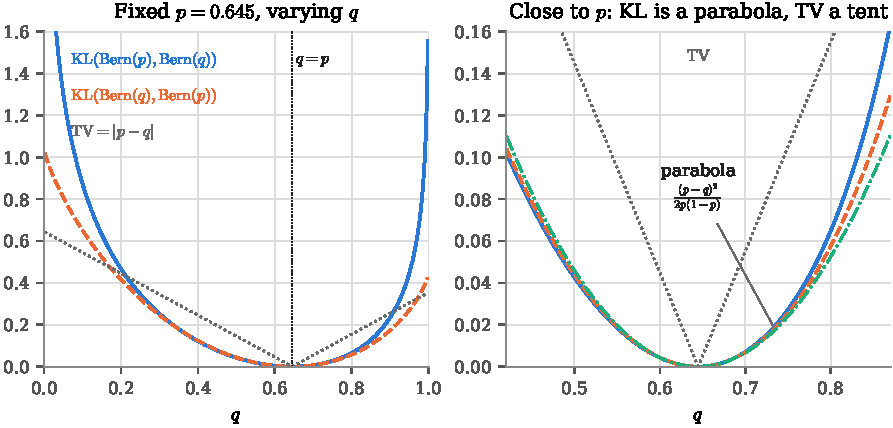
\includegraphics[width=\textwidth]{fig_kl_bernoulli}
\caption{KL divergence and total variation between $\Bern(p)$ and $\Bern(q)$, with $p = 0.645$ fixed and $q$ varying. Left, the whole range: total variation is a tent with straight sides; the two KL divergences are smooth at $q = p$, differ from each other away from it, and $\KL(\Bern(p), \Bern(q))$ (blue) goes to infinity as $q$ approaches $0$ or $1$, where $\Bern(q)$ calls one of the two outcomes impossible. Right, near $q = p$: both KL curves hug the parabola $(p - q)^2 / (2p(1-p))$. At $q = \frac12$: total variation $0.145$, the two KL divergences $0.0428$ and $0.0440$, the parabola $0.0460$.}
\label{fig:klbern}
\end{figure}

\begin{worked}[KL divergences you can compute by hand]
\begin{itemize}
\item \textbf{Two Bernoullis.} With two outcomes the sum has two terms:
\[
\KL(\Bern(p), \Bern(q)) = p \log \frac{p}{q} + (1 - p) \log \frac{1 - p}{1 - q}.
\]
\Cref{fig:klbern} plots it with $p = 0.645$ fixed.
Two values to keep: $\KL(\Bern(\frac12), \Bern(\frac1{10})) = 0.511$ and $\KL(\Bern(\frac1{10}), \Bern(\frac12)) = 0.368$.
\item \textbf{Two Gaussians with the same variance.} For $\Pr = \Gauss(a, \sigma^2)$ and $\Qr = \Gauss(b, \sigma^2)$ the normalizing constants cancel in the ratio, and
\[
\log \frac{p(x)}{q(x)} = \frac{(x - b)^2 - (x - a)^2}{2\sigma^2} = \frac{(a - b)(2x - a - b)}{2\sigma^2}.
\]
This is linear in $x$, so its expectation under $X \sim \Gauss(a, \sigma^2)$ is the same expression at $x = a$:
\[
\KL(\Gauss(a, \sigma^2), \Gauss(b, \sigma^2)) = \frac{(a - b)(2a - a - b)}{2\sigma^2} = \frac{(a - b)^2}{2\sigma^2}.
\]
Half the squared distance between the means in standard-deviation units. For the left pair of \cref{fig:paramvsdist}, means $0$ and $0.01$ with $\sigma = 1$ give $0.00005$. The right pair, standard deviations $0.01$ and $0.02$, does not have a common variance and needs the general formula of \cref{ex:dist-kl-gauss}: $\KL(\Gauss(0, 0.01^2), \Gauss(0, 0.02^2)) = 0.318$, and $0.807$ the other way.
\item \textbf{Two exponentials.} For $\Expo(\lambda)$ against $\Expo(\mu)$, $\log(p(x)/q(x)) = \log(\lambda/\mu) - (\lambda - \mu)x$, again linear in $x$, with $\E[X] = 1/\lambda$:
\[
\KL(\Expo(\lambda), \Expo(\mu)) = \log \frac{\lambda}{\mu} - \frac{\lambda - \mu}{\lambda} = \log\frac{\lambda}{\mu} + \frac{\mu}{\lambda} - 1.
\]
$\KL(\Expo(1), \Expo(2)) = 0.307$ and $\KL(\Expo(2), \Expo(1)) = 0.193$.
\end{itemize}
\end{worked}

\begin{sanitycheck}[The Gaussian formula]
Check $(a - b)^2/(2\sigma^2)$ three ways.
At $a = b$ it is $0$, which a divergence between a distribution and itself must be.
It is symmetric in $a$ and $b$, which is right here (swapping the two Gaussians is the same as reflecting the line, and reflecting changes nothing), though KL is not symmetric in general.
And it is unchanged if $a$, $b$ and $\sigma$ are all converted to a new unit, say minutes instead of hours: a divergence between distributions can't depend on the units of the measurement, and $(a - b)/\sigma$ doesn't.
\end{sanitycheck}

\begin{proposition}[Properties of the KL divergence]
\label{prop:kl-properties}
For distributions $\Pr$ and $\Qr$ on $E$:
\begin{enumerate}[nosep]
\item \textbf{nonnegativity:} $\KL(\Pr, \Qr) \geq 0$;
\item \textbf{definiteness:} $\KL(\Pr, \Qr) = 0$ only if $\Pr = \Qr$;
\item \textbf{no symmetry:} in general $\KL(\Pr, \Qr) \neq \KL(\Qr, \Pr)$;
\item \textbf{no triangle inequality:} in general $\KL(\Pr, \Qr) \not\leq \KL(\Pr, \mathbb{V}) + \KL(\mathbb{V}, \Qr)$.
\end{enumerate}
Properties 1 and 2 make KL behave like a distance in the way that matters most: it is zero exactly when the distributions agree. Properties 3 and 4 mean it is not a distance, which is why it is called a divergence.
\end{proposition}

\coreproof{The log-ratio $\log(p/q)$ is $-\log$ of the ratio $q/p$. The curve $-\log y$ lies above its tangent line $1 - y$ at $y = 1$, touching it only there. The average of the ratio $q(X)/p(X)$ under $\Pr$ is at most $1$, since it is the total mass of $q$ on the points where $p$ is positive, so the average of the tangent line is at least $0$.}
\begin{proof}
(1) If $\KL(\Pr, \Qr) = +\infty$ there is nothing to prove, so assume $q > 0$ wherever $p > 0$.
Let $X \sim \Pr$ and $Y = q(X)/p(X)$, a positive random variable.
Then $\log(p(X)/q(X)) = -\log Y$.
The function $g(y) = -\log y$ is convex ($g''(y) = 1/y^2 > 0$), so it lies above its tangent line at $y = 1$, which is $1 - y$, and touches it only at $y = 1$ \toolkit{sec:math-convex}:
\[
-\log y \geq 1 - y \quad \text{for all } y > 0, \text{ with equality only at } y = 1.
\]
Taking expectations,
\[
\KL(\Pr, \Qr) = \E[-\log Y] \geq 1 - \E[Y].
\]
In the discrete case, $\E[Y] = \sum_{x: p(x) > 0} p(x) \cdot q(x)/p(x) = \sum_{x: p(x) > 0} q(x) \leq 1$; in the continuous case the same with an integral.
So $1 - \E[Y] \geq 0$. (This is the same idea as Jensen's inequality, \cref{thm:jensen}: the tangent-line argument is its proof.)

(2) If $\KL(\Pr, \Qr) = 0$, both inequalities in (1) are equalities.
The first, $\E[-\log Y] = 1 - \E[Y]$, is an average of the nonnegative gap $-\log Y - (1 - Y)$ that comes out $0$, so the gap is $0$ with probability $1$, which forces $Y = 1$: $q(x) = p(x)$ at every point where $p(x) > 0$.
Then $q$ already has total mass $1$ on those points, so it has none anywhere else, and $q = p$.

(3) $\KL(\Bern(\frac12), \Bern(\frac1{10})) = 0.511$ and $\KL(\Bern(\frac1{10}), \Bern(\frac12)) = 0.368$.

(4) With the Gaussian formula,
\[
\begin{aligned}
\KL(\Gauss(0,1), \Gauss(2,1)) &= 2, \quad \text{while}\\
\KL(\Gauss(0,1), \Gauss(1,1)) + \KL(\Gauss(1,1), \Gauss(2,1)) &= 0.5 + 0.5 = 1.
\end{aligned}
\]
The direct route is twice as long as the detour: KL grows like a squared distance, and squares of distances don't satisfy the triangle inequality.
\end{proof}

\begin{intuition}[why the order matters: who is surprised by what]
Think of $\log(1/q(x))$ as how surprised you are to see $x$ if you believe $\Qr$.
Then $\KL(\Pr, \Qr)$ is how much more surprised, on average, a believer in $\Qr$ is than a believer in $\Pr$, when the data really come from $\Pr$.
Take $\Pr = \Bern(\frac12)$, a fair coin, and $\Qr = \Bern(\frac1{10})$, a coin that rarely shows heads.
With the fair coin as the truth, each head is $5$ times likelier under the truth than under $\Qr$, worth $\log 5 = 1.609$ in favor of the truth, and heads come half the time; each tail favors $\Qr$ by $\log(0.9/0.5) = 0.588$.
On average, $0.5 \times 1.609 - 0.5 \times 0.588 = 0.511$.
Reverse the roles, so the $\frac1{10}$ coin is the truth.
Now each tail favors the truth by $0.588$ and comes $90\%$ of the time, while the rare heads favor the fair-coin believer by $1.609$: on average $0.9 \times 0.588 - 0.1 \times 1.609 = 0.368$.
The decisive outcome, heads, is common in the first case and rare in the second.
The divergence is largest when the alternative calls rare what the truth makes common.
At the extreme, $\KL(\Bern(\frac12), \Bern(0)) = +\infty$, since the first head refutes `heads never happen'; but $\KL(\Bern(0), \Bern(\frac12)) = \log 2 = 0.693$, finite, since a stream of tails is perfectly possible for a fair coin, just less likely each time.
\end{intuition}

\subsection{Independent observations add}

The single most useful property of the KL divergence is the one total variation lacks.

\begin{proposition}[Additivity over independent observations]
\label{prop:kl-additive}
If $\Pr^{\otimes n}$ and $\Qr^{\otimes n}$ denote the distributions of $n$ independent draws from $\Pr$ and from $\Qr$, then
\[
\KL(\Pr^{\otimes n}, \Qr^{\otimes n}) = n \, \KL(\Pr, \Qr).
\]
\end{proposition}

\optionalproof{The log of a product is a sum, and an expectation of a sum is a sum of expectations.}
\begin{proof}
The joint PMF or density of $n$ independent draws is the product, so the log-ratio of the joint distributions is a sum:
\[
\log \frac{\prod_{i=1}^n p(x_i)}{\prod_{i=1}^n q(x_i)} = \sum_{i=1}^n \log \frac{p(x_i)}{q(x_i)}.
\]
Under $\Pr^{\otimes n}$ each $X_i \sim \Pr$, and the expectation of a sum is the sum of the expectations, each equal to $\KL(\Pr, \Qr)$.
\end{proof}

Evidence from independent observations accumulates, and on the log scale it accumulates by addition.
For the kiss data, $124$ couples supply on average $124 \times 0.0428 = 5.30$ nats of evidence for $p = 0.645$ over $p = \frac12$, a likelihood ratio of about $e^{5.30} \approx 200$.
The count of right turns is enough to compute that evidence, so the same additivity gives $\KL(\Bin(n, p), \Bin(n, q)) = n\, \KL(\Bern(p), \Bern(q))$, which \cref{ex:dist-kl-binomial} asks you to check directly.
Compare total variation, which went from $0.145$ for one couple to $0.900$ for $124$, by no rule you could state, and could never pass $1$.

\subsection{Near the truth, KL is a parabola}

\Cref{fig:klbern} shows something about the shape of KL that the formulas don't make obvious.
Total variation between Bernoullis is $\abs{p - q}$, a tent with a corner at $q = p$.
KL is smooth there: flat at the bottom, curving up on both sides, the shape of a parabola.
It must be flat at $q = p$, since KL has a minimum of $0$ there and is differentiable.
A second-order Taylor expansion \toolkit{sec:math-mvt} in $q$ around $p$ gives the curvature.
With $f(q) = p \log(p/q) + (1-p)\log((1-p)/(1-q))$, $f(p) = 0$; $f'(q) = -p/q + (1-p)/(1-q)$, so $f'(p) = 0$; and $f''(q) = p/q^2 + (1-p)/(1-q)^2$, so $f''(p) = 1/p + 1/(1-p) = 1/(p(1-p))$.
Hence
\[
\KL(\Bern(p), \Bern(q)) \approx \frac12 f''(p) (q - p)^2 = \frac{(p - q)^2}{2p(1 - p)} \quad \text{for $q$ near $p$}.
\]
For the kiss data the approximation gives $0.0460$ against the exact $0.0428$.

Look at what the curvature is: $1/(p(1-p))$, one over the variance of a single Bernoulli observation.
The Gaussian formula has the same shape, $(a - b)^2/(2\sigma^2)$, with curvature $1/\sigma^2$.
In both, KL near the truth is half the squared parameter distance measured in units of the noise in one observation.
Where an observation is noisy, nearby parameters are hard to tell apart and KL rises slowly; where it is precise, KL rises fast.
\Cref{ch:mle-properties} gives the curvature its name, the Fisher information, and shows that it sets the variance of the best estimators.

\begin{bridge}[the $G$-test and Pearson's chi-squared]
Some introductory courses teach a test of a proportion, or of a table of counts, called the $G$-test or likelihood-ratio chi-squared test: $G^2 = 2\sum O \log(O/E)$, summed over cells, with $O$ the observed and $E$ the expected counts.
That statistic is a KL divergence.
For the kiss data, the cells are right and left, $O = (80, 44)$ and, under $p = \frac12$, $E = (62, 62)$:
\[
G^2 = 2\left(80 \log \tfrac{80}{62} + 44 \log \tfrac{44}{62}\right) = 2 \times 124 \times \KL\big(\Bern(\hat{p}), \Bern(\tfrac12)\big) = 10.60,
\]
twice the $5.30$ nats of evidence above.
Pearson's chi-squared statistic for the same table is $\sum (O - E)^2/E = 10.45$, which is also $z^2 = 3.233^2$ from the test of \cref{sec:tests-kiss}.
Pearson's statistic is a parabola approximation to $G^2$, with the variance taken at the null value.
The expansion above was in $q$ around $p$; expanding instead in $p$ around $q$ gives the same parabola with the variance at $q$, $(p - q)^2/(2q(1 - q))$.
With $q = \frac12$ that is $2(\hat{p} - \frac12)^2 = 0.0421$, and $248 \times 0.0421 = 10.45$, Pearson's statistic.
With the variance at $\hat{p}$ instead, $248 \times 0.0460 = 11.41$, the square of the Wald statistic $\sqrt{124}(\hat{p} - \frac12)/\sqrt{\hat{p}(1 - \hat{p})} = 3.38$ of \cref{ch:wald-lrt}.
Both are compared with a chi-squared distribution with one degree of freedom, whose $95\%$ quantile is $3.84 = 1.96^2$, and both reject.
\Cref{ch:gof} develops the chi-squared test in general.
\end{bridge}

\subsection{KL controls total variation}

KL is not a distance, but small KL forces small total variation.

\begin{theorem}[Pinsker's inequality]
\label{thm:pinsker}
For any distributions $\Pr$ and $\Qr$,
\[
\TV(\Pr, \Qr) \leq \sqrt{\tfrac12 \KL(\Pr, \Qr)}.
\]
\end{theorem}

Nothing later in the book depends on Pinsker's inequality, so its proof is in \cref{sec:proof-pinsker} of \cref{app:proofs}. It is a page of calculus that reuses the tangent-line bound from the proof of \cref{prop:kl-properties}.
For the kiss data, $\sqrt{0.0428/2} = 0.146$, against $\TV = 0.145$: nearly tight.
The inequality is what lets you work with KL, which is convenient, and still conclude something about total variation, which is what you wanted in \cref{sec:dist-close}: if the fitted distribution is close to the truth in KL, then every probability it reports is close to the true probability.
The converse fails: total variation can be small while KL is infinite.
$\Pr = \Pois(1/n)$ and $\Qr$, the distribution that puts all its mass at $0$, have $\TV = 1 - e^{-1/n}$, which goes to $0$, while $\KL(\Pr, \Qr) = +\infty$ for every $n$, since $\Pr$ gives positive probability to $1$ and $\Qr$ calls it impossible (\cref{ex:dist-pois-dirac}).

\section{Estimating the KL divergence: the road to maximum likelihood}
\label{sec:dist-estimating-kl}

Return to the plan of \cref{sec:dist-tv-estimate} with KL in place of total variation.
The quantity to make small is $\theta \mapsto \KL(\Pr_{\theta^*}, \Pr_\theta)$, the divergence of the candidate from the truth.
The truth goes first: the average is taken under the distribution the data come from, which is the only distribution you can average under.
Split the logarithm of the ratio into a difference:
\[
\KL(\Pr_{\theta^*}, \Pr_\theta) = \E_{\theta^*}\big[\log p_{\theta^*}(X)\big] - \E_{\theta^*}\big[\log p_\theta(X)\big].
\]
The first term involves the unknown $\theta^*$, but it does not involve $\theta$: as a function of $\theta$ it is a constant.
The second term is an expectation under the truth of a function, $\log p_\theta$, that you can compute for any $\theta$ you like.

\recall{The Law of Large Numbers (\cref{thm:wlln}): an average of $h(X_1), \ldots, h(X_n)$ over iid data converges in probability to $\E_{\theta^*}[h(X)]$, provided $h(X)$ has finite variance.}

Apply it to $h = \log p_\theta$, one $\theta$ at a time:
\[
\widehat{\KL}(\Pr_{\theta^*}, \Pr_\theta) = \text{constant} - \frac1n \sum_{i=1}^n \log p_\theta(X_i).
\]
You don't know the constant, and you don't need to.
The $\theta$ that minimizes $\widehat{\KL}$ is the same whatever the constant is, and it is the $\theta$ that maximizes $\frac1n \sum_i \log p_\theta(X_i)$.
Since $\log$ turns a product into a sum and is increasing \toolkit{sec:math-explog},
\[
\operatorname*{argmin}_\theta \widehat{\KL}(\Pr_{\theta^*}, \Pr_\theta) = \operatorname*{argmax}_\theta \sum_{i=1}^n \log p_\theta(X_i) = \operatorname*{argmax}_\theta \prod_{i=1}^n p_\theta(X_i).
\]
The product $\prod_i p_\theta(X_i)$ is the probability, or density, of the data you observed, computed as if $\theta$ were the truth.
The $\theta$ that makes your data most probable is the \textbf{maximum likelihood estimator}, and minimizing the estimated KL divergence is the same thing as finding it.
\Cref{ch:likelihood} takes this as its starting point.

\begin{worked}[the kiss data]
For Bernoulli data, $\log p_q(x) = x \log q + (1 - x)\log(1 - q)$, and the average over $124$ couples of whom $80$ turned right is
\[
\frac{1}{124}\sum_{i=1}^{124} \log p_q(R_i) = \hat{p} \log q + (1 - \hat{p}) \log(1 - q), \qquad \hat{p} = \tfrac{80}{124} = 0.645.
\]
Its derivative in $q$ is $\hat{p}/q - (1 - \hat{p})/(1 - q)$, which is zero at $q = \hat{p}$, positive before and negative after.
The estimated KL is smallest at the sample proportion, $\hat{p} = 0.645$, the estimator you would have used anyway.
\end{worked}

\Cref{fig:klestimate} shows the estimate at work.
To draw it, the unknown constant has to be filled in, so the figure does what only a simulation can: it fixes the truth at $p^* = 0.645$ and draws samples from it.
The black curve is the true $\KL(\Bern(p^*), \Bern(q))$.
Each colored curve is the estimate from one simulated sample, $\frac1n \sum_i \log(p^*(R_i)/p_q(R_i))$, the same curve as the true one with the expectation replaced by an average.
Each estimated curve has its minimum at its own sample proportion.
As $n$ grows the estimated curves close in on the true one, and their minimizers close in on $p^*$, which is the true curve's minimizer.
That is the argument \cref{ch:mle-properties} turns into a proof that the maximum likelihood estimator is consistent.

\begin{figure}[htbp]
\centering
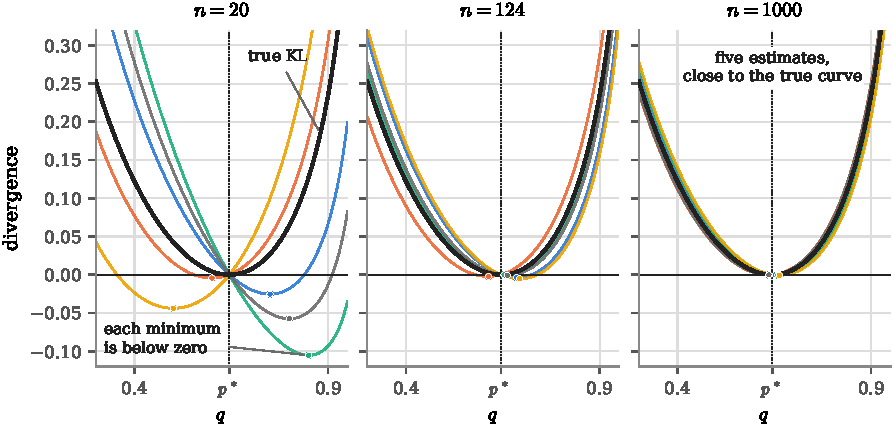
\includegraphics[width=\textwidth]{fig_kl_estimate}
\caption{The true $\KL(\Bern(p^*), \Bern(q))$ for $p^* = 0.645$ (black) and five estimates of it, each from one simulated sample of $n$ couples (colors), for $n = 20$, $124$ and $1{,}000$. Each estimated curve is lowest at its own sample proportion (dots), which is the maximum likelihood estimate. Every estimated curve passes through $0$ at $q = p^*$ and dips below zero near its minimum. As $n$ grows the estimates close in on the true curve, and their minimizers on $p^*$.}
\label{fig:klestimate}
\end{figure}

\begin{sanitycheck}[An estimated divergence below zero]
Every estimated curve in \cref{fig:klestimate} dips below zero, and a KL divergence is never negative.
Is the estimate broken?
No.
At $q = p^*$ the estimate is exactly $0$ (each term is $\log 1$), and at its own minimizer $\hat{p}$ it must be lower still.
The estimate is an average, and an average of quantities whose expectation is positive can come out negative in a finite sample; the LLN promises only that it ends up near the expectation.
What the dip measures is how much better the sample proportion fits this sample than the truth does, which is always at least a little, since $\hat{p}$ was chosen by looking at the sample.
For $n = 20$ the dips are visible; for $n = 1{,}000$ they are invisible at this scale.
\end{sanitycheck}

\begin{pitfall}[the constant you dropped was the distance]
Minimizing $\widehat{\KL}$ finds the best $\theta$, but the minimum value of $-\frac1n\sum_i \log p_\theta(X_i)$ is not an estimate of the distance from the truth.
The dropped constant $\E_{\theta^*}[\log p_{\theta^*}(X)]$ is unknown, so the number you computed is the divergence plus an unknown shift.
The maximized log-likelihood of the kiss data, $80 \log 0.645 + 44 \log 0.355 = -80.6$, says nothing on its own about how well the Bernoulli model fits.
Only differences of log-likelihoods, between two values of $\theta$ or two models fitted to the same data, cancel the constant and mean something.
That is why the likelihood ratio tests of \cref{ch:wald-lrt} compare two maximized log-likelihoods and never interpret one alone.
\end{pitfall}

\section{When the model is wrong: the closest member of the family}
\label{sec:dist-projection}

Everything so far assumed the truth is $\Pr_{\theta^*}$ for some $\theta^*$ in the model.
\Cref{ch:models} warned that the assumption can fail, and promised to say what estimators estimate when it does.
Here is the answer.

Let the truth be any distribution $\Pr$, in the family or not.
\recall{The Law of Large Numbers (\cref{thm:wlln}): for iid data from $\Pr$, $\frac1n \sum_i h(X_i) \convp \E_\Pr[h(X)]$ when $h(X)$ has finite variance. Nothing in it requires $\Pr$ to belong to a model.}
The estimated divergence is built the same way: $\KL(\Pr, \Pr_\theta) = \E_{\Pr}[\log p(X)] - \E_{\Pr}[\log p_\theta(X)]$, the first term is still a constant, and the LLN still estimates the second by $\frac1n\sum_i \log p_\theta(X_i)$, since the data still come from $\Pr$.
So maximum likelihood still minimizes an estimate of $\theta \mapsto \KL(\Pr, \Pr_\theta)$.
What has changed is the minimum: no $\theta$ makes the divergence $0$, so the minimizer is the member of the family that is closest to the truth, not the truth.

\begin{definition}[KL projection]
\label{def:kl-projection}
Let $\Pr$ be a distribution and $(\Pr_\theta)_{\theta \in \Theta}$ a family on the same sample space.
A \textbf{KL projection} of $\Pr$ onto the family is a parameter
\[
\theta^\circ = \operatorname*{argmin}_{\theta \in \Theta} \KL(\Pr, \Pr_\theta),
\]
when the minimum exists and is attained at a single point.
If $\Pr = \Pr_{\theta^*}$ is in the family and the model is identifiable, $\theta^\circ = \theta^*$.
\end{definition}

\begin{inwords}
\textbf{In words.} Look over every distribution the model allows and pick the one the truth diverges from least. If the truth is in the model, that is the truth itself, at divergence $0$. If not, it is the model's best impersonation of the truth. Maximum likelihood, applied to data from a truth outside the model, estimates $\theta^\circ$: under conditions that \cref{ch:mle-properties} states, $\hat{\theta}_n \convp \theta^\circ$. So a wrong model fitted by maximum likelihood is not meaningless. It converges to something definite, the closest member of the family, and the question is only whether the closest member is close enough for your purpose.
\par\smallskip
\textbf{For the kiss data.} The Bernoulli family contains every distribution on $\{0, 1\}$, so for the kiss experiment the model cannot be wrong in this sense: whatever the truth is, one couple's turn is some $\Bern(p)$. What can fail is the iid assumption of \cref{ch:kiss}: couples influencing each other, or one observer's couples differing from another's. A Bernoulli model with dependent data is misspecified in a way that no projection onto a family of iid models repairs.
\end{inwords}

\begin{proposition}[KL projection onto the Gaussian and Poisson families]
\label{prop:kl-projection}
Let $\Pr$ be the distribution of a random variable $X$.
\begin{enumerate}[nosep]
\item If $X$ has a density $p$ with $\E\abs{\log p(X)} < \infty$ and finite variance, the KL projection onto $(\Gauss(\mu, \sigma^2))_{\mu \in \real, \sigma^2 > 0}$ is $\mu^\circ = \E[X]$, $(\sigma^2)^\circ = \var(X)$: the Gaussian with the same mean and variance.
\item If $X$ takes values in $\{0, 1, 2, \ldots\}$, with $\E[X] > 0$, $\E[\log X!] < \infty$ and $\E\abs{\log p(X)} < \infty$ for its PMF $p$, the KL projection onto $(\Pois(\lambda))_{\lambda > 0}$ is $\lambda^\circ = \E[X]$: the Poisson with the same mean.
\end{enumerate}
\end{proposition}

The conditions on $\log p(X)$ keep the constant $\E[\log p(X)]$ finite. Without them the divergence can be $+\infty$ for every member of the family (a discrete $X$ against any Gaussian, say), and what maximum likelihood targets is then the minimizer of $-\E[\log p_\theta(X)]$ alone, which the same calculation finds.

\optionalproof{Only the term $-\E[\log p_\theta(X)]$ depends on the parameter. For both families it involves $X$ only through $\E[X]$ and $\E[X^2]$ (plus a term free of the parameter), so it is an explicit function of the parameters. Minimize it by calculus.}
\begin{proof}
(1) For the Gaussian density, $-\log p_{\mu, \sigma^2}(x) = \frac12 \log(2\pi\sigma^2) + (x - \mu)^2/(2\sigma^2)$, and
\[
-\E[\log p_{\mu,\sigma^2}(X)] = \tfrac12 \log(2\pi\sigma^2) + \frac{\E[(X - \mu)^2]}{2\sigma^2} = \tfrac12 \log(2\pi\sigma^2) + \frac{\var(X) + (\E[X] - \mu)^2}{2\sigma^2},
\]
using the bias-variance split $\E[(X - \mu)^2] = \var(X) + (\E[X] - \mu)^2$ from \cref{ch:estimators}.
For any $\sigma^2$, the $\mu$ that minimizes this is $\mu = \E[X]$, which kills the squared term.
With that $\mu$, the derivative in $\sigma^2$ of $\frac12\log(2\pi\sigma^2) + \var(X)/(2\sigma^2)$ is $\frac{1}{2\sigma^2} - \frac{\var(X)}{2\sigma^4}$, zero at $\sigma^2 = \var(X)$, negative before and positive after, so this is the minimum.

(2) For the Poisson PMF, $-\log p_\lambda(x) = \lambda - x\log\lambda + \log(x!)$, and $-\E[\log p_\lambda(X)] = \lambda - \E[X] \log\lambda + \E[\log X!]$.
The last term doesn't depend on $\lambda$.
The derivative of the rest is $1 - \E[X]/\lambda$, zero at $\lambda = \E[X]$, negative before and positive after.
\end{proof}

\begin{worked}[fitting a Gaussian to exponential data]
Let the truth be $\Expo(1)$, which has mean $1$ and variance $1$, and fit the Gaussian family.
The KL projection is $\Gauss(1, 1)$.
From the proof, with $\var(X) = 1$ and $\E[X] = 1$, and with the constant term $\E[\log e^{-X}] = -\E[X] = -1$,
\[
\KL(\Expo(1), \Gauss(\mu, \sigma^2)) = \tfrac12\log(2\pi\sigma^2) + \frac{1 + (1 - \mu)^2}{2\sigma^2} - 1.
\]
At the projection the divergence is $\frac12\log(2\pi) + \frac12 - 1 = 0.419$.
The minimum is not $0$, since no Gaussian is an exponential.
\Cref{fig:klprojection} shows the projection against two other candidates, $\Gauss(0.7, 0.6)$, which is taller and sits closer to the exponential's peak at $0$, and $\Gauss(1.5, 1.5)$, which covers its long right tail better.
Both diverge more, $0.572$ and $0.538$.
The divergence weights each point by how often the truth produces it, and it penalizes a candidate that calls likely outcomes unlikely; matching the mean and the variance is the best a Gaussian can do on that criterion.
\end{worked}

\begin{figure}[htbp]
\centering
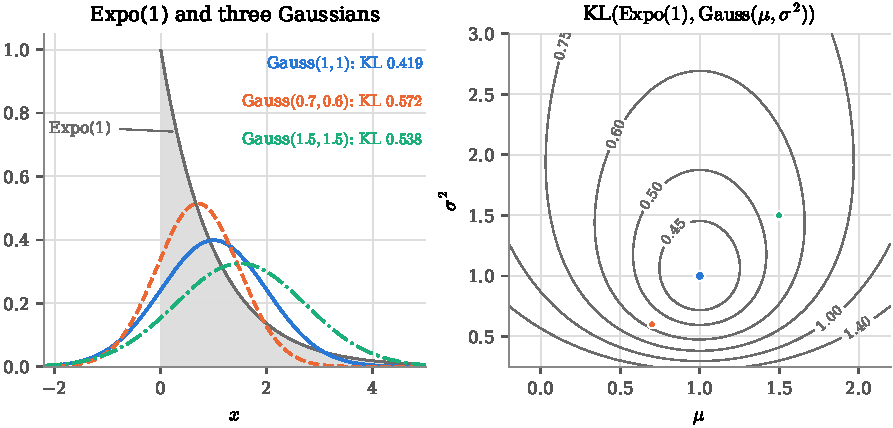
\includegraphics[width=\textwidth]{fig_kl_projection}
\caption{Projecting $\Expo(1)$ onto the Gaussian family. Left: the exponential density (gray) and three Gaussians with their KL divergences from it. Right: $\KL(\Expo(1), \Gauss(\mu, \sigma^2))$ over a grid of means and variances, with its minimum $0.419$ at mean $1$ and variance $1$, the exponential's own mean and variance; the dots mark the three Gaussians on the left.}
\label{fig:klprojection}
\end{figure}

The Poisson half of \cref{prop:kl-projection} pays off the debt of \cref{ch:models}.
The siblings data of \cref{fig:siblings} were fitted with $X - 1 \sim \Pois(\hat{\lambda})$ and $\hat{\lambda}$ the sample mean minus one.
If the true distribution of the number of siblings is not a shifted Poisson, say with an extra bump at $5$, the fit is still estimating something definite: the shifted Poisson whose mean matches the true mean, $\lambda^\circ = \E[X] - 1$, which is the KL projection.
The sample mean minus one estimates it by the LLN, which needs no assumption that the shifted Poisson is right.
Whether that projection is a good description of the truth is a separate question, and it is the question the goodness-of-fit tests of \cref{ch:gof} ask.

\begin{bridge}[`fit a normal with the sample mean and standard deviation']
An introductory course fits a normal distribution to data by plugging in $\bar{x}$ and $s$, and justifies it, if at all, by saying that the normal is determined by its mean and standard deviation.
\Cref{prop:kl-projection} is a better justification, and it holds whether or not the data are normal: $\Gauss(\E[X], \var(X))$ is the Gaussian closest to the truth in KL, and $\bar{x}$ and $s^2$ estimate its two parameters.
What the procedure can't tell you is whether the closest Gaussian is close.
For exponential data it is $0.419$ nats away, and probabilities computed from it can be badly wrong: under $\Gauss(1, 1)$ the probability of a negative value is $\Phi(-1) = 0.16$, under $\Expo(1)$ it is $0$.
A QQ plot (\cref{ch:ks}) is how you see that in data.
\end{bridge}

\begin{pitfall}[the order of the arguments is not a choice]
$\KL(\Pr, \Pr_\theta)$ and $\KL(\Pr_\theta, \Pr)$ are different functions of $\theta$ with different minimizers in general.
Statistics minimizes the first, with the truth first, and not because it is better in some abstract sense: it is the only one that can be estimated.
The first is an expectation under the truth $\Pr$, which the data average.
The second is an expectation under the candidate $\Pr_\theta$, and it has the unknown $p$ inside it in a way that does not split off as a constant.
Because KL is not symmetric, the two orders are different problems, and only the truth-first order is an average under the distribution the data come from.
\end{pitfall}

\section{What comes next}
\label{sec:dist-next}

This chapter ended at maximum likelihood without defining a likelihood.
\Cref{ch:likelihood} defines it, for discrete and continuous models, and computes the maximum likelihood estimator for the families of this book: Bernoulli, Poisson, Gaussian, exponential, uniform.
\Cref{ch:mle-properties} proves what \cref{fig:klestimate} shows, that the estimator converges to the minimizer of the KL divergence, and then uses the curvature of KL at its minimum, the $1/(p(1-p))$ of \cref{fig:klbern}, to find its asymptotic variance: that curvature is the Fisher information.
Distances between distributions return in \cref{ch:ks}, where the largest gap between an empirical CDF and a candidate CDF is the test statistic.

\section{Summary}
\label{sec:dist-summary}

\begin{itemize}[nosep]
\item Closeness should be measured between distributions, not parameters: a parameter difference of $0.01$ is $\TV = 0.004$ for two means with $\sigma = 1$ and $\TV = 0.323$ for standard deviations $0.01$ and $0.02$. A distance between distributions also makes sense when the model is wrong.
\item Total variation: $\TV(\Pr, \Qr) = \max_A \abs{\Pr(A) - \Qr(A)} = \frac12 \sum \abs{p - q}$ (or $\frac12\int$), attained at $\{p > q\}$; the area where one density is above the other; $1 - \TV$ is the shared mass. A true distance with values in $[0, 1]$. $\TV(\Bern(p), \Bern(q)) = \abs{p - q}$; kiss data $0.145$ for one couple, $0.900$ for $124$.
\item The best test of $\Pr$ against $\Qr$ has $\alpha + \beta = 1 - \TV$. For $124$ couples it rejects $p = \frac12$ from $72$ right turns, with $\alpha = 0.0438$ and $\beta = 0.0567$.
\item Total variation ignores the geometry of the sample space: $\TV(X, X + 0.001) = 1$, and a discrete distribution is at distance $1$ from every continuous one, so the CLT is not convergence in total variation.
\item Total variation can't be estimated by an average: written as an expectation under the truth, it has the unknown density inside an absolute value. Plugging in frequencies works for a few discrete outcomes and fails for continuous data.
\item KL divergence: $\KL(\Pr, \Qr) = \E_\Pr[\log(p(X)/q(X))]$, the average evidence per observation for $\Pr$ over $\Qr$; $+\infty$ if $\Qr$ calls impossible what $\Pr$ produces. Nonnegative and zero only for $\Pr = \Qr$ (Jensen), but not symmetric and no triangle inequality. Kiss data: $0.0428$ and, reversed, $0.0440$.
\item Formulas: Bernoulli $p\log(p/q) + (1-p)\log((1-p)/(1-q))$; Gaussians with a common variance $(a - b)^2/(2\sigma^2)$; exponentials $\log(\lambda/\mu) + \mu/\lambda - 1$.
\item KL adds over independent observations: $\KL(\Pr^{\otimes n}, \Qr^{\otimes n}) = n \KL(\Pr, \Qr)$; $124 \times 0.0428 = 5.30$ nats for the kiss data. Near the truth it is a parabola with curvature one over the variance of one observation, $(p - q)^2/(2p(1-p))$ for Bernoulli. $2n\KL$ is the $G^2$ statistic, and its parabola approximation is Pearson's chi-squared.
\item Pinsker: $\TV \leq \sqrt{\KL/2}$; the converse fails.
\item $\KL(\Pr_{\theta^*}, \Pr_\theta)$ is a constant minus $\E_{\theta^*}[\log p_\theta(X)]$, and the LLN estimates the second term by $\frac1n \sum \log p_\theta(X_i)$. Minimizing the estimate is maximizing the likelihood $\prod p_\theta(X_i)$. Kiss data: the minimizer is $\hat{p} = 0.645$.
\item When the model is wrong, maximum likelihood estimates the KL projection, the member of the family closest to the truth. For the Gaussian family it has the true mean and variance; for the Poisson family, the true mean. $\Expo(1)$ projects to $\Gauss(1,1)$ at divergence $0.419$.
\end{itemize}

\section{Exercises}
\label{sec:dist-exercises}

\begin{exercise}
\label{ex:dist-tv-bern}
Compute $\TV(\Bern(\frac12), \Bern(\frac12))$, $\TV(\Bern(\frac12), \Bern(\frac13))$ and $\TV(\Bern(\frac12), \Bern(\frac1{10}))$ from \cref{def:tv}, by listing the events, and check each against the formula $\abs{p - q}$.
\end{exercise}
\begin{solution}
On $E = \{0, 1\}$ the events are $\emptyset$, $\{0\}$, $\{1\}$ and $E$, and the first and last have the same probability under any two distributions. For $\Bern(\frac12)$ against $\Bern(q)$, the event $\{1\}$ has probabilities $\frac12$ and $q$, and $\{0\}$ has $\frac12$ and $1 - q$; both differences are $\abs{\frac12 - q}$. So the three distances are $0$, $\frac16 = 0.167$ and $0.4$, matching $\abs{p - q}$. The first is $0$ whether or not two Bernoulli variables with these distributions are independent: total variation compares distributions, not random variables, and their joint behavior doesn't enter.
\end{solution}

\begin{exercise}
\label{ex:dist-tv-expo-unif}
Show that $\TV(\Expo(1), \Unif([0,1])) = 1/e$, and identify the event $A^\star$ of \cref{prop:tv-area}.
\end{exercise}
\begin{solution}
The computation is the third item of the worked example in \cref{sec:dist-tv}. The event on which $\Expo(1)$ puts more mass is $A^\star = \{x > 1\}$, where the uniform density is $0$; its probabilities are $e^{-1}$ and $0$, so $\abs{\Pr(A^\star) - \Qr(A^\star)} = e^{-1} = 0.368$, the same answer as the integral. The complementary event $[0, 1]$ favors the uniform by the same amount, $1 - (1 - e^{-1}) = e^{-1}$.
\end{solution}

\begin{exercise}
\label{ex:dist-tv-shift}
Let $X \sim \Bern(\frac12)$ and $a \in (0, 1)$. Show that $\TV(X, X + a) = 1$, meaning the total variation distance between the distributions of $X$ and $X + a$. Then show that $\TV(2\sqrt{n}(\bar{X}_n - \frac12), Z) = 1$ for every $n$, where $\Xton \iid \Bern(\frac12)$ and $Z \sim \Gauss(0,1)$, and explain why this does not contradict the CLT.
\end{exercise}
\begin{solution}
$X$ takes values in $\{0, 1\}$ and $X + a$ in $\{a, 1 + a\}$, disjoint from it since $0 < a < 1$. The event $A = \{0, 1\}$ has $\Pr(X \in A) = 1$ and $\Pr(X + a \in A) = 0$, so $\TV = 1$, the largest possible value. For the second, $2\sqrt{n}(\bar{X}_n - \frac12)$ takes values in the finite set $S_n = \{2\sqrt{n}(k/n - \frac12) : k = 0, \ldots, n\}$, so $\Pr(2\sqrt{n}(\bar{X}_n - \frac12) \in S_n) = 1$, while $\Pr(Z \in S_n) = 0$ because a continuous random variable has probability $0$ of landing in any finite set. Hence $\TV = 1$. The CLT says $\Pr(2\sqrt{n}(\bar{X}_n - \frac12) \leq t) \to \Phi(t)$ for every $t$: convergence of the probabilities of the intervals $(-\infty, t]$. Total variation asks for agreement on all events at once, including the finite set $S_n$, which changes with $n$. Convergence in distribution is the weaker requirement.
\end{solution}

\begin{exercise}
\label{ex:dist-best-test}
For one observation from $\Bern(p_0)$ or $\Bern(p_1)$ with $p_0 < p_1$, list all four tests (rejection regions $\emptyset$, $\{0\}$, $\{1\}$, $\{0, 1\}$), compute $\alpha + \beta$ for each, and confirm that the smallest is $1 - \abs{p_1 - p_0}$, as \cref{prop:tv-best-test} says. Evaluate for $p_0 = \frac12$, $p_1 = 0.645$.
\end{exercise}
\begin{solution}
$\alpha = \Pr_{p_0}(R)$, $\beta = \Pr_{p_1}(R^c)$. $R = \emptyset$: $\alpha = 0$, $\beta = 1$, sum $1$. $R = \{0, 1\}$: $\alpha = 1$, $\beta = 0$, sum $1$. $R = \{1\}$: $\alpha = p_0$, $\beta = 1 - p_1$, sum $1 - (p_1 - p_0)$. $R = \{0\}$: $\alpha = 1 - p_0$, $\beta = p_1$, sum $1 + (p_1 - p_0)$. The smallest is $1 - (p_1 - p_0) = 1 - \TV$, from the test that rejects when $X = 1$, the outcome $\Bern(p_1)$ favors. For the kiss values, $0.855$: one couple barely distinguishes the two hypotheses.
\end{solution}

\begin{exercise}
\label{ex:dist-kl-binomial}
Compute $\KL(\Bin(n, p), \Bin(n, q))$ directly from the Binomial PMF and show that it equals $n\,\KL(\Bern(p), \Bern(q))$. Evaluate for $n = 124$, $p = 80/124$, $q = \frac12$.
\end{exercise}
\begin{solution}
The binomial coefficients cancel in the ratio: $\log\big(p_{\Bin(n,p)}(k)/p_{\Bin(n,q)}(k)\big) = k\log(p/q) + (n - k)\log((1-p)/(1-q))$. This is linear in $k$, and under $\Bin(n, p)$, $\E[K] = np$, so the expectation is $np\log(p/q) + n(1 - p)\log((1-p)/(1-q)) = n\,\KL(\Bern(p), \Bern(q))$. For the kiss data, $124 \times 0.0428 = 5.30$. The count of right turns carries the same evidence as the full sequence of turns, which is why the distributions of the sequence and of the count give the same divergence.
\end{solution}

\begin{exercise}
\label{ex:dist-kl-gauss}
Show that
\[
\KL(\Gauss(a, \sigma^2), \Gauss(b, \tau^2)) = \log\frac{\tau}{\sigma} + \frac{\sigma^2 + (a - b)^2}{2\tau^2} - \frac12.
\]
Check that it reduces to $(a - b)^2/(2\sigma^2)$ when $\tau = \sigma$, and evaluate it for $\Gauss(0, 0.01^2)$ against $\Gauss(0, 0.02^2)$ and the other way round.
\end{exercise}
\begin{solution}
The log-ratio of the densities is
\[
\log\frac{p(x)}{q(x)} = \log\frac{\tau}{\sigma} - \frac{(x - a)^2}{2\sigma^2} + \frac{(x - b)^2}{2\tau^2}.
\]
Under $X \sim \Gauss(a, \sigma^2)$, $\E[(X - a)^2] = \sigma^2$ and $\E[(X - b)^2] = \sigma^2 + (a - b)^2$, so the expectation is $\log(\tau/\sigma) - \frac12 + (\sigma^2 + (a-b)^2)/(2\tau^2)$. With $\tau = \sigma$ the first term is $0$ and the rest is $\frac12 + (a - b)^2/(2\sigma^2) - \frac12$. For $\sigma = 0.01$, $\tau = 0.02$, $a = b = 0$: $\log 2 + \frac{1}{8} - \frac12 = 0.318$. The other way round, $\sigma = 0.02$, $\tau = 0.01$: $\log\frac12 + 2 - \frac12 = 0.807$. Believing the narrow distribution when the wide one is true is costlier: the wide one regularly produces values the narrow one calls very unlikely.
\end{solution}

\begin{exercise}
\label{ex:dist-kl-expo}
Show that $\KL(\Expo(\lambda), \Expo(\mu)) = \log(\lambda/\mu) + \mu/\lambda - 1$, check that it is nonnegative by studying $t \mapsto t - 1 - \log t$ with $t = \mu/\lambda$, and check that it is $0$ only when $\lambda = \mu$.
\end{exercise}
\begin{solution}
The derivation is the third item of the worked example in \cref{sec:dist-kl}. With $t = \mu/\lambda > 0$ the divergence is $-\log t + t - 1 = g(t)$. Then $g(1) = 0$, and $g'(t) = 1 - 1/t$ is negative for $t < 1$ and positive for $t > 1$, so $g$ has its minimum $0$ at $t = 1$ and is positive elsewhere. This is \cref{prop:kl-properties} for this family, by direct calculation instead of Jensen.
\end{solution}

\begin{exercise}
\label{ex:dist-pois-dirac}
Let $\Pr_n = \Pois(1/n)$ and let $\delta_0$ be the distribution that puts all its mass at $0$. Compute $\TV(\Pr_n, \delta_0)$, $\KL(\Pr_n, \delta_0)$ and $\KL(\delta_0, \Pr_n)$, and say what happens as $n \to \infty$.
\end{exercise}
\begin{solution}
$\Pr_n$ puts mass $e^{-1/n}$ at $0$ and $1 - e^{-1/n}$ on $\{1, 2, \ldots\}$. By \cref{prop:tv-area}, $\TV = \frac12\big(\abs{e^{-1/n} - 1} + (1 - e^{-1/n})\big) = 1 - e^{-1/n} \to 0$ ($0.095$ at $n = 10$). $\KL(\Pr_n, \delta_0) = +\infty$ for every $n$, since $\Pr_n$ gives positive probability to $1$, which $\delta_0$ calls impossible. $\KL(\delta_0, \Pr_n)$ has a single term, at $x = 0$: $1 \cdot \log\big(1/e^{-1/n}\big) = 1/n \to 0$. So $\Pr_n$ approaches $\delta_0$ in total variation and in one direction of KL, and stays infinitely far in the other.
\end{solution}

\begin{exercise}
\label{ex:dist-kl-mle-poisson}
Let $\Xton \iid \Pois(\lambda^*)$. Write $\widehat{\KL}(\Pois(\lambda^*), \Pois(\lambda))$ up to its constant, and find the $\lambda$ that minimizes it.
\end{exercise}
\begin{solution}
$\log p_\lambda(x) = -\lambda + x\log\lambda - \log(x!)$, so $\widehat{\KL} = \text{constant} - \frac1n\sum_i \log p_\lambda(X_i) = \text{constant}' + \lambda - \bar{X}_n\log\lambda$, where $\frac1n\sum_i\log(X_i!)$ has been absorbed into the constant since it doesn't depend on $\lambda$. The derivative $1 - \bar{X}_n/\lambda$ is zero at $\lambda = \bar{X}_n$, negative before and positive after. The minimizer, which is the maximum likelihood estimator, is the sample mean. It is the sample version of \cref{prop:kl-projection}(2), with the true mean replaced by the sample mean.
\end{solution}

\begin{exercise}
\label{ex:dist-projection-bin}
Data $X_i \in \{0, 1, 2\}$ come from a distribution with $\Pr(X = 0) = 0.5$, $\Pr(X = 1) = 0.2$, $\Pr(X = 2) = 0.3$, and are fitted with the model $X \sim \Bin(2, \theta)$. Find the KL projection $\theta^\circ$ and the divergence at it. Is the model well-specified?
\end{exercise}
\begin{solution}
$-\E[\log p_\theta(X)] = -\E[\log\binom{2}{X}] - \E[X]\log\theta - (2 - \E[X])\log(1 - \theta)$, and only the last two terms depend on $\theta$. Setting the derivative $-\E[X]/\theta + (2 - \E[X])/(1 - \theta)$ to zero gives $\theta^\circ = \E[X]/2 = (0.2 + 0.6)/2 = 0.4$: the Binomial with the same mean. $\Bin(2, 0.4)$ has PMF $(0.36, 0.48, 0.16)$, and $\KL = 0.5\log(0.5/0.36) + 0.2\log(0.2/0.48) + 0.3\log(0.3/0.16) = 0.164 - 0.175 + 0.189 = 0.178$. The model is not well-specified: every $\Bin(2, \theta)$ satisfies $\Pr(X = 1)^2 = 4\Pr(X = 0)\Pr(X = 2)$, and here $0.04 \neq 0.6$. The fitted model matches the mean but puts far too much mass on $1$ and too little on $0$ and $2$.
\end{solution}
